% !TeX spellcheck = de_DE
\documentclass{uebung_cs}
\usepackage{algo123}
\uebung{6}{}{}
\blattname{Gerichtete Graphen}

\usepackage{etoolbox}\AtBeginEnvironment{algorithmic}{\small}
\newcommand{\fett}[1]{\textbf{\boldmath\color{red!60!black}#1}}

%%%%%%%%%%%%%%%%%%%%%%%%%%%%%%%%%%%%%%%%%%%%%%%%%%%%%%%%%%%%%%%%%%%%%%%%%%%%


\begin{document}
\textbf{Eigenständige Vorbereitung:}\\
Lies \emoji{book} CLRS Einleitung Teil VI, Kapitel 22.1--22.4, sowie Appendix B.4--B.5 und schau dir das \emoji{television} Video der Woche an.

\textbf{Zeichenlegende:}
\legende{}

%  \schriftlich
%  \bestehen
%  \mittel
%  \note
%  \spass

\begin{aufgabe}[Darstellung, Eigenschaften und Algorithmen]
	Löse für die Graphen in Abbildung~\ref{digraph} folgende Aufgaben:
	\begin{enumerate}
		\item (\warmup) Zeige die Adjazenzlisten und Adjazenzmatrizen für Graph (a) und Graph (b).
		\item (\warmup) Führe die Breitensuche und Tiefensuche in den Graphen (a) und (c) aus.
		Die Startknoten sind \textbf{Knoten 4 in Graph (a)} und \textbf{Knoten 5 in Graph (c)}
		\item Welcher der Graphen (a) und (c) ist ein gerichteter azyklischer Graph?
		Wenn ein Graph ein gerichteter azyklischer Graph ist, finde mithilfe des rekursiven Algorithmus für das topologische Sortieren eine topologische Ordnung der Knoten.
		Finde ansonsten einen Kreis.
		\item Gib die stark zusammenhängenden Komponenten der Graphen (a) und (c) an.
		\item Wie viele verschiedene topologische Ordnungen hat Graph (b)?
		\item Wie viele stark zusammenhängende Komponenten hat ein gerichteter azyklischer Graph?
	\end{enumerate}
\end{aufgabe}

\begin{center}
	\begin{figure}[h]
		\begin{subfigure}[b]{0.33\textwidth}
			\hspace*{\fill}
			\scalebox{0.7}
			{
				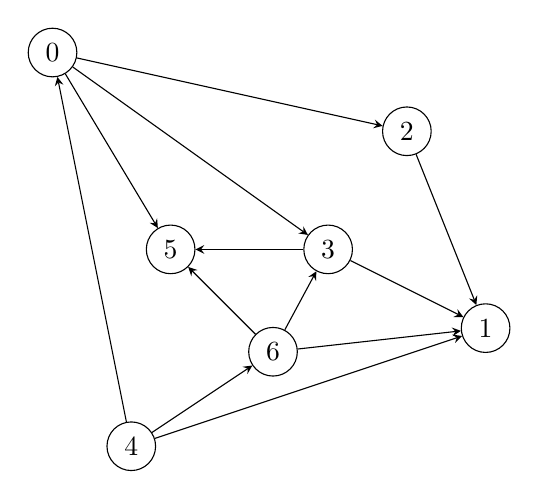
\begin{tikzpicture}
					\node[draw,circle] (v0) at (0,5)     {$0$};
					\node[draw,circle] (v1) at (5.5,1.5) {$1$};
					\node[draw,circle] (v2) at (4.5,4)   {$2$};
					\node[draw,circle] (v3) at (3.5,2.5) {$3$};
					\node[draw,circle] (v4) at (1,0)     {$4$};
					\node[draw,circle] (v5) at (1.5,2.5) {$5$};
					\node[draw,circle] (v6) at (2.8,1.2) {$6$};
					%
					\draw[-stealth] (v0) -- (v2);
					\draw[-stealth] (v0) -- (v3);
					\draw[-stealth] (v0) -- (v5);
					%
					\draw[-stealth] (v2) -- (v1);
					%
					\draw[-stealth] (v3) -- (v1);
					\draw[-stealth] (v3) -- (v5);
					%
					\draw[-stealth] (v4) -- (v0);
					\draw[-stealth] (v4) -- (v1);
					\draw[-stealth] (v4) -- (v6);
					%
					\draw[-stealth] (v6) -- (v1);
					\draw[-stealth] (v6) -- (v3);
					\draw[-stealth] (v6) -- (v5);
				\end{tikzpicture}
			}
			\caption{}
			\hspace*{\fill}
		\end{subfigure}
		\begin{subfigure}[b]{0.33\textwidth}
			\hspace*{\fill}
			\scalebox{0.7}
			{
				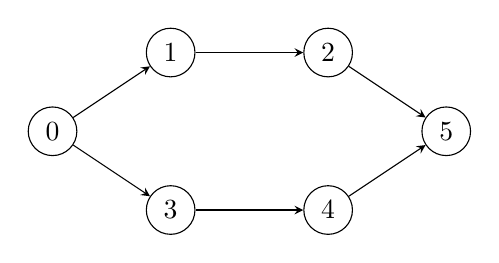
\begin{tikzpicture}
					\node[draw,circle] (v0) at (0.5,2) {$0$};
					\node[draw,circle] (v1) at (2,3)   {$1$};
					\node[draw,circle] (v2) at (4,3)   {$2$};
					\node[draw,circle] (v3) at (2,1)   {$3$};
					\node[draw,circle] (v4) at (4,1)   {$4$};
					\node[draw,circle] (v5) at (5.5,2) {$5$};
					%
					\draw[-stealth] (v0) -- (v1);
					\draw[-stealth] (v1) -- (v2);
					\draw[-stealth] (v2) -- (v5);
					\draw[-stealth] (v0) -- (v3);
					\draw[-stealth] (v3) -- (v4);
					\draw[-stealth] (v4) -- (v5);
				\end{tikzpicture}
			}
			\caption{}
			\hspace*{\fill}
		\end{subfigure}
		\begin{subfigure}[b]{0.33\textwidth}
			\hspace*{\fill}
			\scalebox{0.6}
			{
				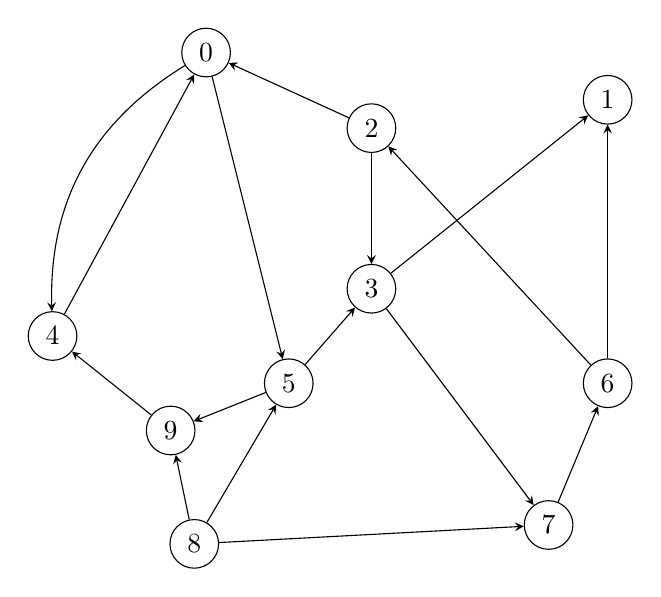
\begin{tikzpicture}
					% scale parameters
					\def\xscale {1.5};
					\def\yscale {1.2};
					% node labels
					\def\labels {4,9,8,5,0,2,3,1,6,7};
					% node xy coordinates
					\def\pos { (\xscale * 0   , 0     * \yscale)
							 , (\xscale * 1   , -1    * \yscale)
							 , (\xscale * 1.2 , -2.2  * \yscale)
							 , (\xscale * 2   , -0.5  * \yscale)
							 , (\xscale * 1.3 ,  3    * \yscale)
							 , (\xscale * 2.7 ,  2.2  * \yscale)
							 , (\xscale * 2.7 ,  0.5  * \yscale)
							 , (\xscale * 4.7 ,  2.5  * \yscale)
							 , (\xscale * 4.7 , -0.5  * \yscale)
							 , (\xscale * 4.2 , -2    * \yscale)
							 };
					% draw nodes and labels
					\foreach \coords [count=\index] in \pos
					{
						% node (v_\index) at \coords {\index};  % uncomment for debugging
						\node[draw, circle] (v_\index) at \coords {\phantom{0}};
					}
					\foreach \label [count=\index] in \labels
					{
						\node () at (v_\index) {\label};  % comment for debugging
					}
					% edges
					\draw[-stealth] (v_1) -- (v_5);
					\draw[-stealth] (v_2) -- (v_1);
					\draw[-stealth] (v_3) -- (v_2);
					\draw[-stealth] (v_3) -- (v_4);
					\draw[-stealth] (v_3) -- (v_10);
					\draw[-stealth] (v_4) -- (v_2);
					\draw[-stealth] (v_4) -- (v_7);
					\draw[-stealth] (v_5) -- (v_4);
					\draw[-stealth, bend right=30] (v_5) to (v_1);
					\draw[-stealth] (v_6) -- (v_5);
					\draw[-stealth] (v_6) -- (v_7);
					\draw[-stealth] (v_7) -- (v_8);
					\draw[-stealth] (v_7) -- (v_10);
					\draw[-stealth] (v_9) -- (v_8);
					\draw[-stealth] (v_9) -- (v_6);
					\draw[-stealth] (v_10) -- (v_9);
				\end{tikzpicture}
			}
			\hspace*{\fill}
			\caption{}
		\end{subfigure}
		\caption{\label{digraph}Drei gerichtete Graphen.}
	\end{figure}
\end{center}

\begin{aufgabe}[Rolltreppen und Aale]
	\emph{Rolltreppen und Aale} ist ein klassisches Brettspiel (manchmal auch als \emph{Schlangen und Leitern} bekannt).
	Wir schauen uns die folgende Variante an.
	Das Spielbrett ist ein $n \times n$ Feld mit Zellen, die von $1$ bis $n^2$ in der Reihenfolge nummeriert sind, wie in Abbildung~\ref{snakesladders} dargestellt.
	Bestimmte Zellpaare sind Aale (\emph{rote Pfeile}), die nach unten führen, oder Rolltreppen (\emph{blaue Pfeile}), die nach oben führen.
	Eine Zelle kann nur der Endpunkt für \textbf{entweder} einen Aal \textbf{oder} eine Rolltreppe sein.

	Das Ziel des Spiels ist es, sich von Zelle $1$ zu Zelle $n^2$ in möglichst wenig Runden zu bewegen.
	Als Erstes wird eine Spielfigur auf das Feld $1$ platziert.
	In jeder Runde kann die Figur um maximal $5$ Zellen nach vorne verschoben werden.
	Wenn die Figur am oberen Ende eines Aals ankommt, wird sie zum unteren Ende dieses Aals bewegt.
	Genauso wird eine Figur, die am unteren Ende einer Rolltreppe ankommt, an ihr oberes Ende bewegt.
	
	Entwerfe einen Algorithmus, der die geringste Anzahl an Runden berechnet, die benötigt werden, um eine Spielfigur von Zelle $1$ zu Zelle $n^2$ zu bewegen.
\end{aufgabe}
\begin{figure}[h]
	\begin{center}
		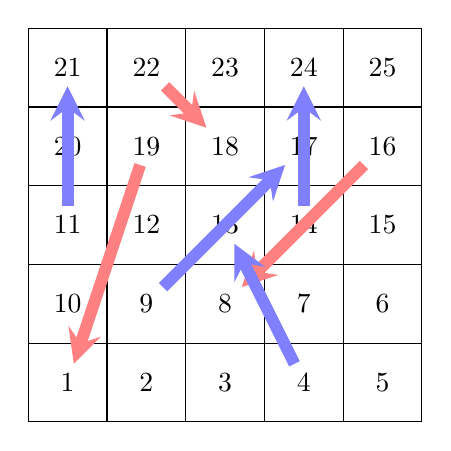
\begin{tikzpicture}
			\draw (0,0) grid (5,5);

			\foreach \x in {1,...,5}
			{
				\node (n_\x) at (\x - 0.5, 0.5) {\x};
			}
			\foreach \x in {6,...,10}
			{
				\node (n_\x) at (10.5 - \x, 1.5) {\x};
			}
			\foreach \x in {11,...,15}
			{
				\node (n_\x) at (-10.5 + \x, 2.5) {\x};
			}
			\foreach \x in {16,...,20}
			{
				\node (n_\x) at (20.5 - \x, 3.5) {\x};
			}
			\foreach \x in {21,...,25}
			{
				\node (n_\x) at (-20.5 + \x, 4.5) {\x};
			}

			\draw [-stealth, red!50, line width=1.5mm] (n_19) to (n_1);
			\draw [-stealth, red!50, line width=1.5mm] (n_22) to (n_18);
			\draw [-stealth, red!50, line width=1.5mm] (n_16) to (n_8);

			\draw [-stealth, blue!50, line width=1.5mm] (n_11) to (n_21);
			\draw [-stealth, blue!50, line width=1.5mm] (n_9) to (n_17);
			\draw [-stealth, blue!50, line width=1.5mm] (n_4) to (n_13);
			\draw [-stealth, blue!50, line width=1.5mm] (n_14) to (n_24);
		\end{tikzpicture}
	\end{center}
		\caption{\label{snakesladders}Rolltreppen und Aale}
	\end{figure}
\begin{aufgabe}[Gerichtete azyklische Graphen und topologische Sortierung]\mbox{}
	\begin{enumerate}
		\item Professorin Tina Opologisch schlägt folgenden neuen und einfachen Algorithmus zur Bestimmung einer topologischen Ordnung vor: Führe eine Breitensuche von einem Knoten $s$ mit Ein-Grad $0$ aus und sortiere die Knoten aufsteigend nach dem Abstand zu s. Funktioniert dieser Algorithmus?
		\item Bestimme einen Algorithmus, der als Eingabe einen Graphen $G$ und eine Reihenfolge $S$ der Knoten in $G$ erhält und bestimmt, ob $S$ eine topologische Ordnung für $G$ ist.
		\item Gegeben ist ein gerichteter, azyklischer Graph $G$.
		Gibt es eine topologische Ordnung von~$G$, die nicht durch den rekursiven Algorithmus gefunden werden kann?
		\item (\hard) Ein Hamilton-Weg ist ein Weg, der jeden Knoten genau einmal besucht.
		Bestimme einen Algorithmus, der feststellt, ob ein gerichteter, azyklischer Graph einen Hamilton-Weg enthält.
	\end{enumerate}
\end{aufgabe}

\begin{aufgabe}[Studiengangplanung]
Algolina hat den gesamten Sommer damit verbracht, sich zu überlegen, welche Kurse sie an der Universität der Algorithmen belegen möchte.
Der Abschluss eines Kurses benötigt ein Semester. Sie ist zwar eine Super-Studentin und besteht jeden Kurs, aber manche Kurse hängen von anderen Kursen ab und die Universität erlaubt es nicht, solche Kurse im selben Semester zu belegen. Wenn Kurs $i$ von Kurs $j$ abhängt, muss Algolina Kurs $j$ in einem früheren Semester als Kurs $i$ belegen.
Sie möchte ihr Studium in möglichst wenigen Semestern abschließen.

Gegeben sind $N$ Kurse (nummeriert von $1$ bis $N$), die Algolina belegen möchte, und die jeweiligen Kurse von denen diese abhängen.
Ermittle die geringste Anzahl an Semestern, die Algolina braucht, um ihr Studium abzuschließen.
(Da Algolina eine Super-Studentin ist, kann sie unendlich viele Kurse pro Semester belegen.)
Es kann angenommen werden, dass es keine zyklischen Abhängigkeiten gibt.
Bestimme einen Algorithmus, um dieses Problem zu lösen. Implementiere diesen Algorithmus.
\end{aufgabe}


\begin{aufgabe}[Ethnographen, \hard]
Du hilfst einer Gruppe von Ethnographen bei der Analyse mündlicher Geschichtsdaten, die sie durch die Befragung von Dorfbewohner:innen gesammelt haben. Das Ziel der Studie war es, mehr über das Leben von den Menschen zu erfahren, die in den letzten zweihundert Jahren in dem Dorf gelebt haben.

In den Interviews haben die Ethnographen herausgefunden, dass es eine Menge von $n$ mittlerweile verstorbenen Personen gab, die als $P_1, P_2, \ldots, P_n$ notiert sind.
Sie haben zudem Fakten darüber gesammelt, wann diese Menschen im Verhältnis zueinander gelebt haben. Jeder Fakt ist in einer der folgenden beiden Formen aufgeschrieben:
\begin{enumerate}
	\item Für ein $i$ und ein $j$: Person $P_i$ starb bevor $P_j$ geboren wurde.
	\item Für ein $i$ und ein $j$: Die Lebensdauer von $P_i$ und $P_j$ überlappen zumindest teilweise.
\end{enumerate}
Natürlich sind sich die Ethnographen nicht sicher, ob all diese Fakten korrekt sind; Erinnerungen sind nicht immer verlässlich und Vieles wurde nur mündlich weitergegeben.

Du sollst nun ermitteln, ob die Daten zumindest untereinander konsistent sind.
Das heißt es kann eine Menge an Menschen gegeben haben, für die alle gesammelten Fakten gleichzeitig wahr sind.
Bestimme einen effizienten Algorithmus, der diese Aufgabe löst: entweder sollte er Geburts- und Todesdatum für alle $n$ Menschen ausgeben, sodass alle gesammelten Fakten wahr sind, oder wenn dies nicht möglich ist, ausgeben, dass die Fakten, die die Ethnographen gesammelt haben, untereinander nicht konsistent sind. 
\end{aufgabe}


\begin{aufgabe}[Topologische Sortierung und gerichtete azyklische Graphen]
Zeige, dass ein gerichteter Graph G genau dann ein gerichteter, azyklischer Graph ist, wenn G eine topologische Ordnung hat.
\textit{Tipp: Nutze das Lemma für die Korrektheit des rekursiven Algorithmus der topologischen Sortierung}
\end{aufgabe}


\begin{aufgabe}[Drei Flaschen]
Du hast drei Flaschen mit einer Kapazität von 8, 5 und 3 Litern.
Zu Beginn ist die 8 Liter Flasche mit Wasser gefüllt und die anderen beiden sind leer.
Dein Ziel ist es, am Ende genau 4 Liter in einer der Flaschen zu haben. Du kannst dafür Wasser von einer Flasche in eine andere gießen, aber musst so lange weitermachen, bis entweder die Flasche, aus der du das Wasser entnimmst, leer ist oder die Flasche, in die du es füllst, voll ist.
Es kann kein Wasser nachgefüllt oder ausgeschüttet werden.
\begin{enumerate}
	\item (\hard) Zeige, dass das möglich ist. Gib die geringste Anzahl an Füllungen/Leerungen von Flaschen an, die du finden kannst.
	\item (\hard) Nimm nun an, dass du $n$ Flaschen mit einer Kapazität von $d_1, \ldots, d_n$ Litern hast und ein Zielvolumen von $x$ Litern Wasser, die am Ende in einer der Flaschen sein soll.
	Zu Begin ist nur die Flasche mit dem größten Volumen gefüllt.
	Es kann kein Wasser nachgefüllt oder ausgeschüttet werden.\\
	Bestimme einen Algorithmus, um die geringste Anzahl an Füllungen/Leerungen von Flaschen zum Erreichen des Zielvolumens zu bestimmen.
	\textit{Tipp: Modelliere das Problem als impliziten Graphen.}
\end{enumerate}
\end{aufgabe}

\begin{aufgabe}[Palindromische Wege \schriftlich]
  \textit{\footnotesize For an English version of this exercise, see [\href{https://jeffe.cs.illinois.edu/teaching/algorithms/book/Algorithms-JeffE.pdf}{Erickson}, page 222]}.

  Ein \emph{Palindrom} über dem Alphabet $\{\texttt{R},\texttt{B}\}$ ist eine Zeichenkette $s_1,s_2,s_3,\dots,s_n\in\{\texttt{R},\texttt{B}\}$, sodass $s_i=s_{n-i+1}$ für alle $i\in\{1,\dots,n\}$. Zum Beispiel sind \texttt{BRBRB} und \texttt{RBBR} Palindrome, aber \texttt{RBB} und \texttt{BRRR} nicht.
  
  Sei $G$ ein beliebiger gerichteter Graph, in dem jede Kante entweder rot oder blau gefärbt ist, und seien $s,t$ zwei Knoten.
  \begin{enumerate}
      \item Beschreibe einen Algorithmus, der entweder einen Weg von $s$ nach $t$ berechnet, für den die Sequenz von rot und blau entlang der Kanten des Weges ein Palindrom ist, oder korrekterweise feststellt, dass kein solcher Weg existiert.
      \item Beschreibe einen Algorithmus, der entweder einen \emph{kürzesten} Weg von $s$ nach $t$ berechnet unter allen Wegen, für die die Sequenz von rot und blau entlang der Kanten des Weges ein Palindrom ist, oder korrekterweise feststellt, dass kein solcher Weg existiert.
  \end{enumerate}
  
\end{aufgabe}

\end{document}
